\chapter{Literature Review}
\section{GPS}
\subsection{History of GPS}
\begin{figure}
	\begin{center}
		\includegraphics[width = 0.65\textwidth]{figures/historyGPS.jpg}
		\caption{Early GPS receivers were large, heavy devices. \cite{USAF1978}}
		\label{fig:2:histGPS}
	\end{center}
\end{figure}
Global Positioning System (GPS) is an everyday thing in our lives today and has become a luxury that most take for granted. There is GPS in our phones, laptops and even cars. We are using it to find directions on our commutes, hail taxis or ride shares and even for recreational sport, tracking how far we travelled.\par
\vspace{0.6cm}
The origins of GPS or rather any global satellite navigation system begins with the space race. It starts, in 1957, with the first satellite to successfully orbit the earth, the Russian satellite Sputnik. During its orbiting flight of the earth, Sputnik was emitting a radio signal which could be picked up on earth. During this orbit Scientists from John Hopkins University in America were monitoring the radio signals emitted by the Sputnik satellite when they saw the Doppler Effect in action with the radio signals, as the satellite drew closer, the radio signal frequency increased and vice versa. These scientists theorized that if they could determine the location of the satellite based on its signal frequency, the opposite would also be true, they could determine the location of a receiver on the ground given the satellites location. \cite{Aerospace2021}\par
\vspace{0.6cm}
The first instance of a global satellite navigation system was the Transit. It was developed in 1958 by the Advanced Research Projects Agency and the first satellite was launch in 1960. The Transit satellites were mostly used by the military, specifically the Navy's missile submarines. The program was transferred to the Navy during the mid-1960s. During this time there were further Transit satellites launched and by 1968 the entire constellation of Transit satellites was operational, a total of 36 satellites. \cite{Aerospace2021}\par
\vspace{0.6cm}
There was plenty of other research that was being conducted around the same time to improve on the current Transit. One such researcher was Phillip Diamond. Diamonds concept, from his study in 1963, lead to the Air Force forming a new satellite navigation program which he called 621-B. Further studies were undertaken by James Woodford and Hideyoshi Nakamura, which completed in 1966, proposed using four satellites. The use of four satellites would mean that the receivers no longer needed to be equipped with high-accuracy clocks. This was the first step in reducing the size and cost of the receivers. \cite{Aerospace2021} \par
\vspace{0.6cm}
There was a range of technological advancements that help progress the satellite navigation systems such as new bandwidth utilization techniques, advancements in computer and the introduction of solid-state microprocessors. These technological advancements helped reduce the size and weight of the GPS receivers to what we now know today, figure \ref{fig:2:histGPS} shows how large and cumbersome the early GPS receivers were. However, one significant technological advancement was the development of atomic clocks. This development led to another satellite navigation system known as Timation (Time Navigation). The third of three Timation satellites launched in 1974, became the first satellite equipped with an atomic clock, the previous two contained crystal oscillator clocks. The use of the atomic clock led to vast improvements in the accuracy of the navigation system and provided three-dimensional location coverage. \cite{Aerospace2021} \par
\vspace{0.6cm}
There were now three satellite navigation systems, and so when in the 1970s, the Department of Defence wanted a robust and stable system, the project team developed a new concept by cherry-picking the best aspects of all three, Transit, Timation and 621-B. This system was designated, Navigation System with Timing and Ranging (NAVSTAR), this was later changed to GPS I, the precursors to the GPS system we know today. The first NAVSTAR satellite was launched in 1978 and further satellites were launched in the following years, the system reaching its fully operational state with 24 satellites in 1993. \cite{Mai2017}\par
\vspace{0.6cm} 
Although the satellite navigation systems were operational and orbiting the earth, they were still used mostly by the military and the receivers were expensive. However, this began to change in 1983 when President Ronald Reagan authorized commercial airlines use of the NAVSTAR system. This was the start of civilian use of GPS. \cite{HistGPSProgram}
\par
\vspace{0.6cm} 
\subsection{Modern GPS}
The cost of GPS receivers began to decrease in the late-1990s, early-200s, the first cell phone containing GPS technology was released in 1999. The cost reduction can be attributed to the American government approving more non-military singnals as well as the technological advances in processors that was leading to cheaper processing chips. And naturally from the cheaper access, GPS use began to grow and putting more tax on the system which although upgraded to GPS II was not equipped to handle the modern requirments. In 2000 a plan was formed to add new signals to satellites that had not yet been launched in order to handle the increased use. Furhtermore, a new system was to be developed, GPS III, that could fully meet the modern requirements. The first of the GPS III satellites was launched in 2018 with a couple more in the following years and the remaining 6 to be launched by 2023. \cite{Aerospace2021}
\subsection{How GPS works}
\begin{figure}
	\begin{center}
		\includegraphics[width = 0.5\textwidth]{figures/GPStriangle.png}
		\caption{Distance spheres around each satellite intersect at one point}
		\label{fig:2:tiangleGPS}
	\end{center}
\end{figure}
There are a total of 31 GPS satellites currently sitting in a medium earth orbit. These are the satellites that are sending the radio signals that a GPS receiver can use to determine its location.\par
\vspace{0.6cm}
The signal that the satellites broadcast has a range of information that is used by receivers, this information contains data needed to determine the location of the satellite as well as the time that the signal broadcast, using the satellites atomic clock. Based on the time taken for the signal to reach the receiver and corrected for propagation delays or delays from the signal passing through the ionosphere and troposphere, the receiver can calculate the distance between itself and the satellite. This creates a sphere around the satellite upon which the receiver must lie. By adding in a second and third satellite and their distance spheres, there will be only two points of intersection between the three spheres. The one will be the receiver's location, while the other will be impossible location in space. However, to accurately calculate the distance, the receiver would have to have a synchronized atomic clock to determine exactly how long the signal takes to reach it. As it was mentioned earlier, highly accurate clocks were taken out of the receivers by adding a measurement from a fourth satellite to ensure that the distance calculation is accurate. Figure \ref{fig:2:tiangleGPS} illustrates the concept of the distance spheres and their intersection being the location of the GPS receiver. \cite{FederalAviationAdministration}
\section{Digital Compass}
Compasses have been used extensively over the past centuries for navigating, surveying, and map-making. The compass is thought to have been in use from around the 12th century in Europe and possibly earlier in east Asia \cite{Jones2019}. Although as many things have over the years been digitalized, so has the compass. The digital compass uses a technology called magneto-induction. This allows the digital compass to electronically detect the earth's magnetic field. Being as sensitive as it is an embedded microcontroller is needed to filter out any magnetic fields from ferro-magnetic materials or other electrical systems that are creating a magnetic field. \cite{AdvancedSafetyDevices2013}
\subsection{What is magnetic north}
\begin{figure}
	\begin{center}
		\includegraphics[width = 0.65\textwidth]{figures/tiltedDipole.jpg}
		\caption{The differentiation between magnetic and true north}
		\label{fig:2:magNorth}
	\end{center}
\end{figure}
True north is always fixed and is the direction that is directly in line with the north pole. However, compasses do not point to true north, they point to magnetic north. This is because a compass aligns itself with the magnetic field caused by the earth's magnetic core. The distinction between true north and the magnetic field at magnetic north is shown in figure \ref{fig:2:histGPS}. To further complicate the matter however, the earth's magnetic core experiences changes and these cause small shifts in the magnetic field around the earth. \cite{Jones2019}
\section{PWM}
\begin{figure}
	\begin{center}
		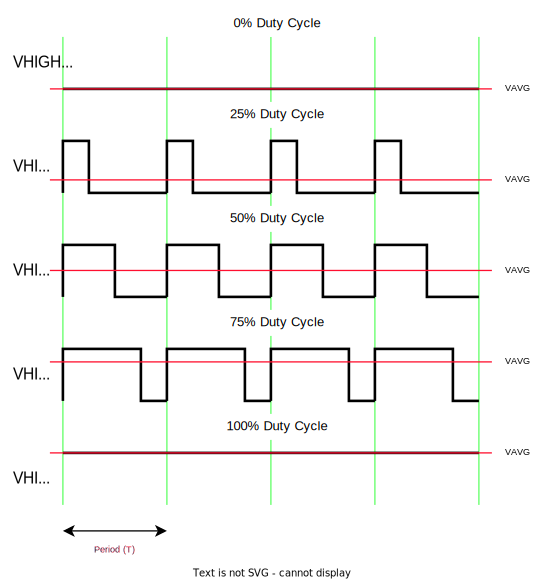
\includegraphics[width = 0.5\textwidth]{figures/PWM.jpg}
		\caption{Duty Cycle of PWM Signal}
		\label{fig:2:PWM}
	\end{center}
\end{figure}
Pulse Width Modulation (PWM) is a technique of using a digital signal to represent an analogue signal which is used to control analogue systems. The cost of switching a digital circuit between on (high) and off (low) is a cheaper alternative to creating an analogue circuit that will incur not drift over time. These PWM signals are mostly used in speed control of DC motors or controlling the brightness of lightbulbs. \cite{Christ2014}\par
\vspace{0.6cm}
PWM is a digital signal that is switched between high and low, leading to the generation of a square wave signal. The time that the signal goes high can be modulated to vary the power delivered to the system. Typically, microcontrollers are used to generate and control the PWM to power an external system. There are a few signal parameters that will be highlighted in this explanation of a PWM signal. The signal amplitude, this is the maximum voltage that can be supplied to the external system. If the microcontrollers output voltage is insufficient for the external system, the signal can be passed through an amplifying circuit to provide the required voltage. Secondly is the signal period, and therefore the frequency as they are inversely proportional, and is the total time for one signal wave to propagate. The frequency is set depending on the requirements of the system, but this frequency will be needed later to help with the calculation of the duty cycle. The duty cycle is the final parameter. The duty cycle is the ratio between the time the signal is high and the time the signal is low. It is always a value between 0 and 1, however, the duty cycle is often expressed as a percentage.\par
\vspace{0.6cm}
A PWM varies the voltage supplied to the system by varying the duty cycle. A small duty cycle means that the signal is high for a short portion of the signal period while a large duty cycle means that the signal is low for a large portion of the signal period. The system that is being supplied then uses the average voltage of this period. Therefore, a low duty cycle, a short high signal followed by a long low signal, would lead to a low average voltage. The variation in duty cycle and the associated average voltage is shown in figure \ref{fig:2:PWM}. \cite{Ibrahim2014}\par
\vspace{0.6cm}
To determine how long the signal must go high, the duty cycle is multiplied by the signal period. The duty cycle is often expressed as a percentage and so the duty cycle is the percentage of time that the signal is high. Therefore, by multiplying the duty cycle with the period gives the time for which the signal is pushed high (t1). Figure \ref{fig:2:PWMPulse} shows the relationship between t1, the time the signal is high, and T, the signal period.\par
\vspace{0.6cm}
\begin{figure}
	\begin{center}
		\includegraphics[width = 0.65\textwidth]{figures/PulseWideWave.jpg}
		\caption{The relation between the time the signal is high and the signal period.}
		\label{fig:2:PWMPulse}
	\end{center}
\end{figure}
\section{Analogue vs Digital Signals}
\begin{figure}
	\begin{center}
		\includegraphics[width = 0.75\textwidth]{figures/DigitalSignal.jpg}
		\caption{A digital signal and its three zones.}
		\label{fig:2:digital}
	\end{center}
\end{figure}
Signals are used to convey data and information from point to point. For this project only electrical signals will be used although there are plenty of other mediums through which signals can be sent. There are two predominant signals that are used when regarding electrical signals, analogue and digital. \par
\vspace{0.6cm}
A digital signal, most simply represents discrete values, more precisely 2 discrete values. This makes digital signals perfect for conveying data in a binary data format but slightly more troublesome when more than two values are required. It will transmit a signal as either a low voltage, a zero, or a high voltage, a one. The low voltage is generally 0V while the high voltage is the voltage supply of the driving device. However, because voltages can have small fluctuations and will therefore not always be exactly 0V or equal to the nominal voltage, a range is pre-set whereby the receiving device can denote the value as low or high. A buffer zone is also incorporated, a voltage range around half the value of the nominal voltage, to prevent a small fluctuation in the voltage possibly altering the value of the signal. This buffer zone along with the area in which the signal can be read as high or low is shown in figure \ref{fig:2:digital}. This buffer is called the forbidden zone any signal received within the forbidden zone is considered floating and will be randomly assigned as either high or low.\par
\vspace{0.6cm}
An analogue signal on the other hand is continuous and where the digital signal ranged from 0 to an upper voltage, an analogue signal ranges from a low voltage to a high voltage. Typically, $±V_CC$, the voltage of the microcontroller, is used for these upper and lower limits. An example of a continuous analogue signal between $±V_CC$ is shown in figure \ref{fig:2:analogue}. An analogue signal can therefore transmit an infinite number of values between these limits. By assigning an upper and lower limit to the sensor that will transmit the data, a max min transformation can be computed, and the transformed value transmitted along the analogue signal. Because the analogue signal is continuous, it can also be used in tracking the change in a value over time by computing the integral of the signal wave.\par
\begin{figure}
	\begin{center}
		\includegraphics[width=0.75\textwidth]{figures/AnalogSignal.jpg}
		\caption{Analogue signal}
		\label{fig:2:analogue}
	\end{center}
\end{figure}


